\chapter[Documentación de programación]{Documentación técnica de programación}

\section{Introducción}
En este apartado vamos a proceder a describir la documentación referente a la programación, incluyendo la instalación del entorno de trabajo o la estructura de la aplicación.

\section{Estructura de directorios}
La estructura de directorios se encuentra distribuida de la siguiente forma:
\begin{itemize}
	\item \textbf{/:} Contiene una copia de la licencia, el fichero README así como el fichero \emph{.gitignore}.
	\item \textbf{/code:} Contiene todos los ficheros referentes al código fuente de la aplicación
	\item \textbf{/md:} Contiene los ficheros referentes a los \emph{Sprints} que se han ido realizando a lo largo del desarrollo del proyecto.
	\item \textbf{/UnitTest:} Contiene los ficheros referentes a los test unitarios que corroboran el correcto funcionamiento de esta.
	\item \textbf{/Doc:} Contiene los ficheros referentes a la documentación del proyecto.
	\item \textbf{/Doc/img:} Contiene las imágenes que han sido utilizadas en la documentación.
	\item \textbf{/Doc/tex:} Contiene los diferentes apartados de los que se componen la memoria y los anexos.
\end{itemize}

\section{Manual del programador}\label{instalar}
Este apartado tiene como objetivo facilitar las labores de futuros programadores que deseen continuar con el trabajo de desarrollo de esta aplicación. Aquí se explica cómo montar el entorno de trabajo, obtener el código de la aplicación, ejecutarlo y ejecutar los test creados.
Para trabajar con este proyecto se necesitan los siguiente programas y librerías:
\begin{itemize}
	\item Python.
	\item pip.
	\item Scholarly.
	\item Bibtexparser.
	\item Selenium.
	\item PIL
\end{itemize}
\subsection{Python}
\emph{Python} es la piedra angular sobre la que está escrito el proyecto, por eso es de imperiosa necesidad tenerlo instalado para continuar con el desarrollo. Aunque durante el desarrollo se usó la versión \emph{3.7.1} actualmente ya existe la versión \emph{3.7.2}, la cual puede ser utilizada sin problemas pues no supone riesgo con la compatibilidad del resto de módulos o librerías.
Para instalarlo basta con acceder a la página oficial de \emph{Python}\cite{python_descargas} , elegir adecuadamente el sistema operativo para el cual se desea instalar, descargar el asistente de instalación  , ejecutar y seguir los pasos que este indica.

En los siguientes enlaces se muestra una ayuda para la instalación en caso de que quedara alguna duda. \cite{python_w10}\cite{python_allos}

\subsection{pip}
\emph{pip} es una poderosa herramienta que facilita considerablemente la vida a la hora de descargar e instalar las librerías para \emph{Python} y será usado como el método principal para instalar las siguientes librerías necesarias. Es por eso que recomiendo fervientemente su descarga y uso.

Para saber como proceder a la hora de instalar esta herramienta, existe un artículo que resumen perfectamente esta labor para todo tipo de sistemas operativos.\cite{pip}
\subsection{Scholarly}
Para instalar la librería \emph{Scholarly}, basta con abrir la consola de comandos y teclear el siguiente comando:\\ \\
\emph{pip install scholarly}

\subsection{Bibtexparser}
Para instalar la librería \emph{Bibtexparser}, basta con abrir la consola de comandos y teclear el siguiente comando:\\ \\
\emph{pip install bibtexparser}

\subsection{Selenium}
Para instalar la librería \emph{Selenium}, basta con abrir la consola de comandos y teclear el siguiente comando:\\ \\
\emph{pip install selenium}

\subsection{PIL}
Para instalar la librería \emph{PIL}, basta con abrir la consola de comandos y teclear el siguiente comando:\\ \\
\emph{pip install Pillow}
\section{Compilación, instalación y ejecución del proyecto}
Tanto para la instalación como la ejecución del proyecto es necesario obtener el repositorio de la plataforma en la que esta alojada (GitHub), para ello basta con acceder a este enlace\cite{github}. A continuación basta con presionar el botón que se encuentra en la parte derecha \emph{Clone or download} :
\begin{figure}[H]
	\centering
	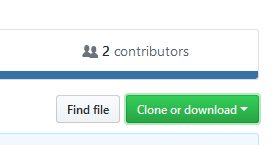
\includegraphics[width=0.4\textwidth]{github_clone}
	\caption{Botón \emph{clone or Download}}
	\label{fig:clone}
\end{figure}
Después tenemos dos opciones clonarlo en nuestro repositorio \emph{git} si tenemos esta herramienta o descargarlo como \emph{ZIP} para después descomprimirlo. Personalmente la última opción es la que recomiendo.
\subsection{Instalación}
Para comenzar a trabajar en el código de esta aplicación no se requiere ningún tipo de instalación, solo es necesario tener las librerías correspondientes instaladas.
\subsection{Ejecución}\label{ejecutar}
Para ejecutar la aplicación basta con ejecutar el archivo \emph{GUI.py}. Para ello necesitamos acceder a a la línea de comandos, desplazarnos hasta el directorio en el que este situado el repositorio y ejecutar el fichero con el comando\\ \\
\emph{python GUI.py}
\section{Pruebas del sistema}
Para verificar el funcionamiento de los módulos de la aplicación se han desarrollado una serie de tests.
\subsection{Test unitarios}
Para el desarrollo de los \emph{Test unitarios} se ha utilizado la propia librería que viene incluida en \emph{Python} con este fin \emph{Unittest}.
Se han implementado un total de 3 test unitarios que prueban el correcto funcionamiento de las funciones definidas en los módulos. Para la ejecución de estos test basta con situarse en la carpeta en la que están contenidos y ejecutar el siguiente comando:\\ \\
\emph{python -m unittest}
